To enhance the summarizer's ability to produce summaries that provide the evidence needed for fact-checking claims, we adopt the concept of training a language model using feedback with reinforcement learning. After pretraining the perceiver and summarization models, we employ reinforcement learning with an entailment model serving as a surrogate for a human fact-checker as feedback. We first exclusively apply reinforcement learning (RL) to the perceiver. Subsequently, we unfreeze the summarizer and continue training end-to-end with both the perceiver and summarizer. We illustrate our fine-tuning process in Figure~\ref{fig:rl_ppo}. Contrary to the approach in reinforcement learning from human feedback, which necessitates a human arbitrator to score the model's outputs, in this study, we train a reward model to act like a human fact-checker to guide the summarizer in producing summaries for fact-checking instead.

\begin{figure*}
  \centering
  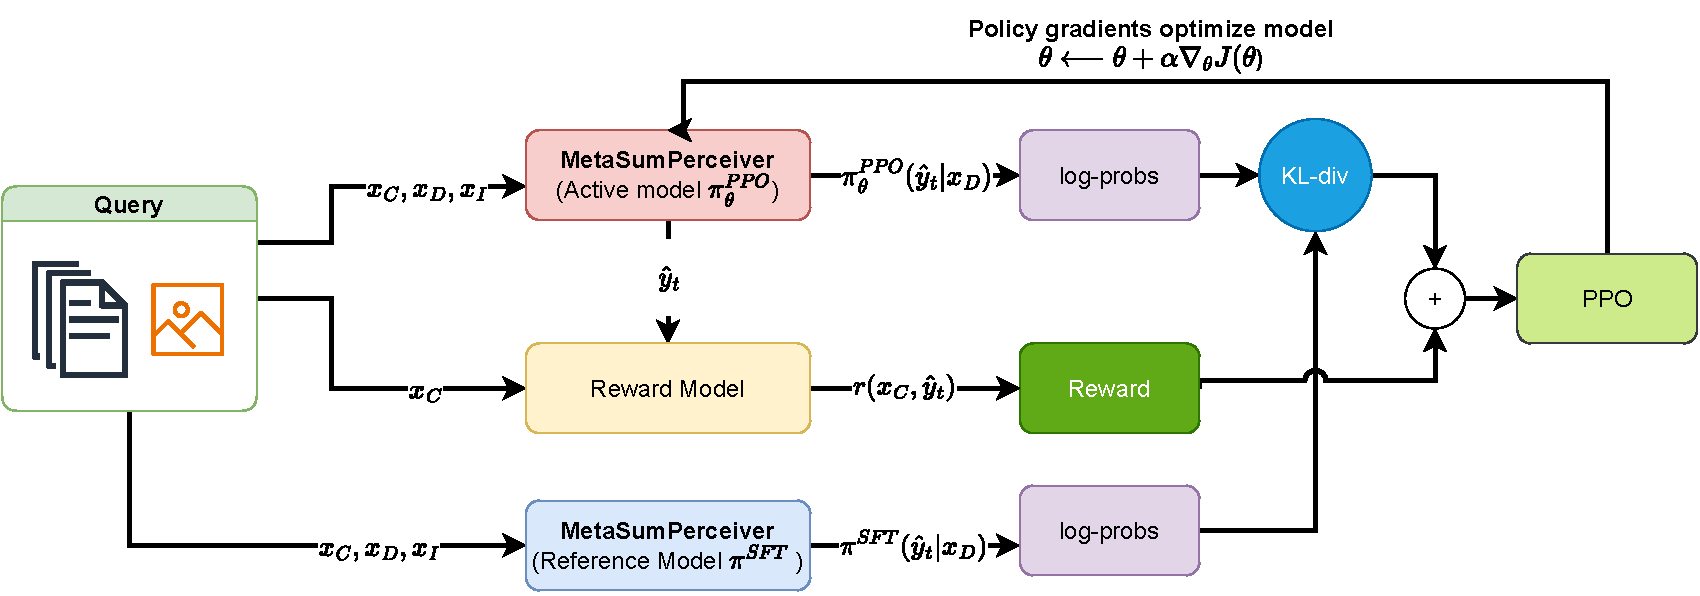
\includegraphics[width=\textwidth,height=\textwidth,keepaspectratio]{images/ppo.pdf}
  \caption{The Proximal Policy Optimization (PPO) workflow begins with the summarizer creating a response based on the input query. The reward model then evaluates this query-response pair that outputs a scalar reward. Meanwhile, the process calculates the KL-divergence based on the likelihood of token sequences in the response using both an active model being fine-tuned currently and a pre-trained reference model. The KL-divergence serves as a reward measure, ensuring responses from the active model are aligned with the reference model. Conclusively, PPO updates the active model's parameters, relying on the result of the reward model's output and the KL-divergence's value.}
  \label{fig:rl_ppo}
\end{figure*}

We utilized a comprehensive dataset consisted with MultiNLI~\cite{N18-1101}, Fever-NLI~\cite{Thorne18Fever}, and Adversarial-NLI (ANLI)~\cite{nie-etal-2020-adversarial}, encompassing a total of 763,193 premise-claim pairs. Leveraging this dataset, we fine-tuned DeBERTa V3~\cite{he2023debertav3} for the task of entailment classification using cross-entropy loss. Serving as an entailment classifier, this model achieves accuracy rates of 90.3\%, 77.7\%, and 57.9\% in the MultiNLI, Fever-NLI, and ANLI evaluation datasets, respectively. We define the score from the reward model as the probability of the ground-truth label given both the claim (as the hypothesis) and the generated summary for fact-checking (as the premise). The formulation for the score from the reward model can be formulated as:

\begin{equation}
  \begin{array}{l}
    r(x_C, \hat{y}_t) = P(y_{gt}|{x_C, \hat{y}_t}) - 
    0.5 * \Sigma_{y_{gt} \neq y_{pred}} P(y_{pred}|{x_C, \hat{y}_t}),
  \end{array}
\end{equation}

where $x_C$, $\hat{y}_t$, $y_{gt}$ and $y_{pred}$ denote the claim, the generated summary, the groud-truth label of the claim, and the predicted label of the claim, respectively. The value of $P(y_{\{gt,pred\}}|x_C,\hat{y}_t)$ is derived from the trained entailment classifier. The primary objective behind this reward function is to maximize the likelihood that the generated summary for fact-checking contains the facts necessary for the model to predict the claim's ground truth label.

We employ PPO as our policy gradient method for reinforcement learning. PPO adds an additional term to the reward function, which imposes a penalty determined by the Kullback-Leibler (KL) divergence between the trained RL policy summarizer, $\pi^{PPO}_{\phi}$, and the initial supervised summarizer $\pi^{SFT}$. This cumulative reward is described as follows:

\begin{equation}
  \begin{array}{l}
    r_{total} = r(x_C, \hat{y}_t) - 
    \eta KL(\pi^{PPO}_{\phi}(\hat{y}_t|x_D), \pi^{SFT}(\hat{y}_t|x_D)),
  \end{array}
\end{equation}

where $\eta$ represents the KL reward coefficient, which determines the magnitude of the KL penalty, we set it to 0.2 for our model. This coefficient functions as an entropy boost, enhancing exploration throughout the policy domain and urging the model to engage in a diverse set of actions rather than the one currently considered the best. In addition, it inhibits the policy from rapidly committing to a singular strategy, and this encourages outputs from the RL fine-tuned model to not deviate too far from the original model. ~\textbf{MetaSumPerceiver} is optimized through PPO based on the policy gradient methods that optimize the policy of the model using gradient ascent. The update rule for the policy gradient is given as: 

\begin{equation}
  \begin{array}{l}
    \theta \longleftarrow \theta + \alpha \nabla_{\theta} J(\theta),
  \end{array}
\end{equation}

where $\alpha$ and $J_{\theta}$ denote the learning rate and the expected return under policy $\pi_{\theta}$ from the model, respectively.


